\documentclass[11pt]{article}
\usepackage[margin=.78in]{geometry}\usepackage{amsmath,amssymb,graphicx,booktabs,hyperref}
\setlength{\parindent}{0pt}\setlength{\parskip}{6pt}
\begin{document}
{\LARGE Complete size-three factor bases over $\mathbf F_{37}$}\\
2026-10-30\quad PR2381\quad fixed public synthetic inputs

The existing actual route is $E:y^2=x^3+7x+19$ to its nonsquare $d=35$
monic twist $T:y^2=x^3+28x+33$. The checked coordinate maps give
$P=(1,8)\mapsto U=(32,29)$ and inverse $[10]D$ on the cyclic subgroups of order 19.
These are exact unregistered model tuples, not invented registry aliases.
\begin{center}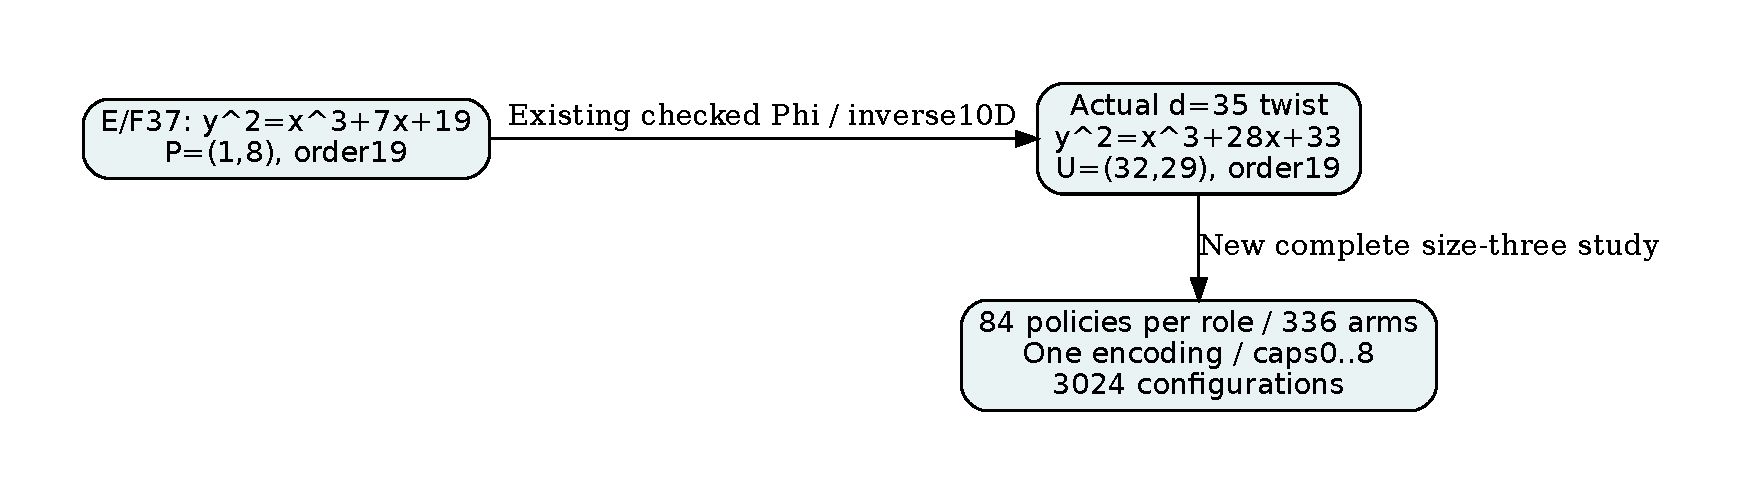
\includegraphics[width=\linewidth,height=1.65in,keepaspectratio]{bridge.pdf}\end{center}

The new cohort contains all size-three subsets of nine unsigned subgroup
abscissae: 84 canonical policies per curve, plus every matched and pullback
control. All 336 arms run caps 0--8 under one original encoding. The 3024
configurations make 54432 separate target attempts on 18 repeated source points.
These are not 54432 distinct DLP challenges.

\textbf{Encoding control.} $S_3$ has degree at most two in each coordinate,
although its total degree is four. Reducing it by a cubic product-membership
polynomial in either coordinate leaves it unchanged. The producer checks the
coefficient bounds; independent Rust performs monic division and checks equality
on every query. A second identical encoding is not counted as an extra arm.

\textbf{New Lean check.} The unmodified scoped gate passes six public named
statements / seven audited declarations, zero failing or extra trusted/native
axioms. Over a nontrivial commutative ring it proves cubic monicity/degree,
the univariate degree bound for the explicit $S_3$, remainder identity, both
coordinate versions and binding to the native value formula. Other coordinates
are parameters. This is an input-equality theorem, not a solving-degree,
intrinsic-regularity or DLP-hardness theorem. The actual source-DLP reduction
uses the earlier F37 19-named/22-audited receipt within its cyclic domain;
that receipt is not a newly combined audit.

\begin{center}\begin{tabular}{lr}\toprule
Independent native outcome & Count\\\midrule
Configurations &3024\\
Verified original-source recovery runs &1944\\
Blocked public-log setups &2916\\
Capped diagnostic query records &52100\\
Policy/target/requested-cap pair records &10287648\\
Strict higher-rank/lower-cap recovery-admitted records &0\\
Such records beating strongest source policy &0\\
Changed controls rejected 101/no receipt &10\\
Shared backend tests passed &22\\\bottomrule\end{tabular}\end{center}

\clearpage
{\Large Recorded outcomes and limits}
\begin{center}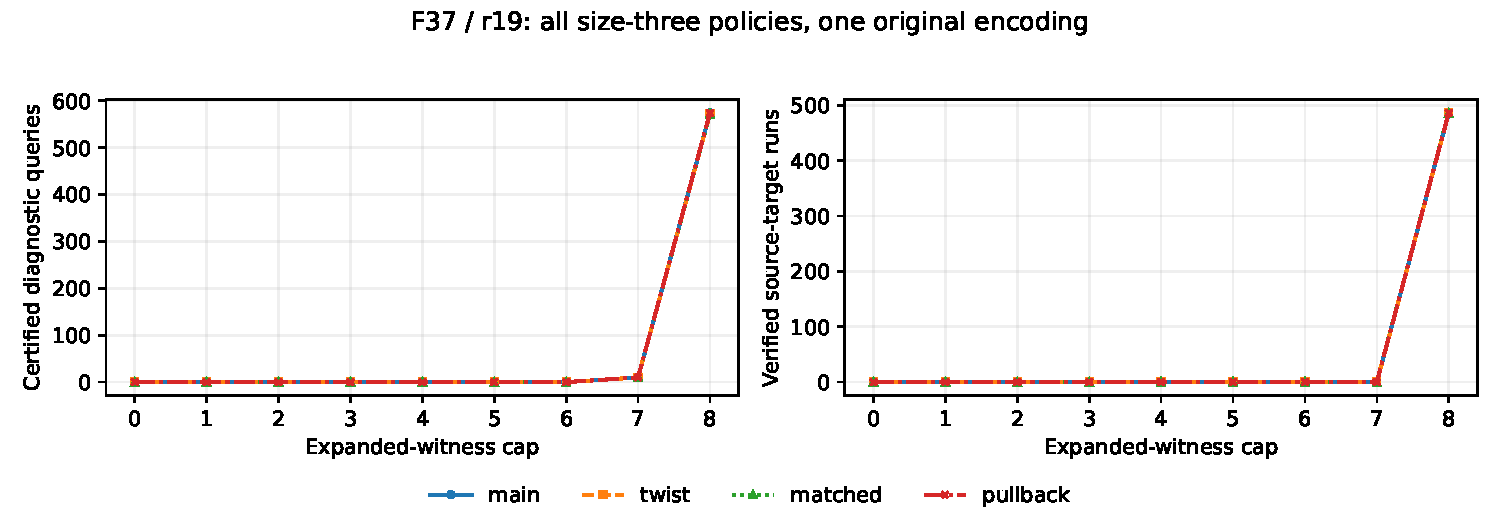
\includegraphics[width=\linewidth]{frontier.pdf}\end{center}
\textbf{Figure.} Native-emitted counts only: 84 policies and 18 source points per
role and cap. Curves may overlap. These are exact finite counts; no timing,
uncertainty estimate or cross-size performance ratio is inferred.

Public setup derives logs only from admitted rows until coefficient rank three,
then checks each base point. Incomplete rank blocks every target. Recovery
receives actual unknown $Q$, uses fresh shifted solves, retains failed and
identity shifts and all ordered sign lifts, and verifies the scalar on original
$E/P$. The finite recovery count repeats the same 18 source points.

The new solver uses $S_3$ and two cubic memberships. Matrix and expanded
original-input verification-witness degrees must fit the rung before shifts
are constructed. A complete unit or bounded Buchberger certificate precedes
root extraction; unknown caps admit no roots or rows. A smaller already-found
witness is retained only for an identical polynomial within one solve.
Independent arithmetic reconstructs every case, witness, row, rank, setup log,
shift and source scalar. A separate degree-free point reference never controls
candidate stopping. Diagnostic output binding follows fresh solves and is
unpriced. Setup, field/group operations, allocation and verification lack a
complete price.

Both full native paths pass. False inverse plus nine genuinely changed/rehashed
case controls reject 101 without receipts. The same 22 backend tests pass.
All four native panels record zero recoveries at caps 0--7 and 486 per role at
cap 8. Hence no admitted target has a higher source comparison cap available
inside 0--8. The zero joint count is boundary-limited, not a proof of universal
no-advantage. The lower cap is a requested budget, not automatically
an actual solving degree. Stationary useful yield, intrinsic regularity and
calibrated complete-cost gains remain open.

\clearpage
{\Large Preservation, integration and next lead}

All cases and altered payloads remain source-bound. Raw sources, commands,
exits, failures and proof receipts are archived. Full control trees reconstruct
from canonical case files plus exact overlays/removals; their bytes match the
originals. Canonical protocol and export hashes bind the new full scope.

Native stages and launcher explicitly record zero; an outer PTY result reported
one despite the explicit file. All stage/rejection receipts and ordinary
metadata checks resolve the distinction without a repeated study. Lean attempt 01
fails on abstract-polynomial computability and ambiguous binomial notation.
Attempt 02 fails on multiplication order and an unmatched section end. Same
statements fixed by a noncomputable section, disambiguated syntax, ring proof
and explicit section closure pass on attempt 03. Failed sources/logs remain;
no sorry or trust bypass is accepted.

\textbf{Owner merge review.} A new normal main merge leaves every frozen study
path unchanged. Active registry records increase 20787 to 20809 by 22 additions,
with no old record removed or shared value changed; the 1921 lost study rows
remain absent. The PR native-audit failure again finds 1921 proposed rows and 3842
aliases. Its actual checkout is a synthetic merge 26fb0d38\ldots, not the literal
PR head; their registry hashes are distinguished. Existing 42 metadata tests and
seven separate replay jobs pass. Required checks are assessed on each resulting
head; older passes do not replace them.

The owner re-enabled auto-merge. A dedicated non-merge GraphQL mutation restored
the user's keep-open state. A CLI spelling was rejected by automatic approval
review before execution. The local fast-forward initially ran out of disk;
only reproducible build cache was removed. Every partial file was verified
against the owner tree before checkout repair. No user changes or evidence
were lost. Root/catalog/naming/coordination/review holds remain.

\textbf{Next test, not executed.} Preregister fresh caps 9--12 across all 336
arms. Retain 0--8 as fixed historical evidence, explicitly separating old and new
executions. This creates comparisons above the observed cap 8 admission boundary;
it must not silently change this frozen contract. Preserve all blocked/failed
setups and the full 84-policy source frontier. A symmetric-coordinate membership
encoding with distinct-root and diagonal branches is a secondary hypothesis:
equivalence, lifting and degree accounting need proof before any such run.
Neither extension nor new encoding is implemented or executed here.

Scientific window 15:15--16:15 UTC: two existing local workers, 600-second command
caps, no paid resources or arbitrary result upload. Keep the same PR open,
non-draft, with auto-merge off. The original stronger goal remains open.
\small Full proof map, exact hypotheses, native receipts, source links,
restoration commands and canonical flow are in the adjacent README/validation.
\end{document}
